%%%%%%%%%%%%%%%%%%%%%%%%%%%%%%%%%%%%%%%%%%%%%%%%%%%%%%%%%%%%%%%%%%%%%%%%%%%%%%%%
\chapter{Building graphs with bundled edges and vertices}
%%%%%%%%%%%%%%%%%%%%%%%%%%%%%%%%%%%%%%%%%%%%%%%%%%%%%%%%%%%%%%%%%%%%%%%%%%%%%%%%

Up until now, the graphs created have had only bundled vertices.
In this chapter, graphs will be created, in which both the edges and vertices
have a bundled \verb;my_bundled_edge; and \verb;my_bundled_edge; type
\footnote{I do not intend to be original in naming my data types}.

\begin{itemize}
  \item An empty directed graph that allows for bundled edges and vertices: 
    see chapter \ref{subsec:create_empty_directed_bundled_edges_and_vertices_graph}
  \item An empty undirected graph that allows for bundled edges and vertices: 
    see chapter \ref{subsec:create_empty_undirected_bundled_edges_and_vertices_graph}
  \item A two-state Markov chain with bundled edges and vertices: 
    see chapter \ref{subsec:create_bundled_edges_and_vertices_markov_chain}
  \item $K_{3}$ with bundled edges and vertices: 
    see chapter \ref{subsec:create_bundled_edges_and_vertices_k3}
\end{itemize}

In the process, some basic (sometimes bordering trivial) functions are shown:

\begin{itemize}
  \item Creating the \verb;my_bundled_edge; class: 
    see chapter \ref{subsec:my_bundled_edge}
  \item Adding a bundled \verb;my_bundled_edge;: 
    see chapter \ref{subsec:add_bundled_edge}
\end{itemize}

These functions are mostly there for completion and showing which data types
are used.

%%%%%%%%%%%%%%%%%%%%%%%%%%%%%%%%%%%%%%%%%%%%%%%%%%%%%%%%%%%%%%%%%%%%%%%%%%%%%%%%
\section{Creating the bundled edge class}
\label{subsec:my_bundled_edge}
%%%%%%%%%%%%%%%%%%%%%%%%%%%%%%%%%%%%%%%%%%%%%%%%%%%%%%%%%%%%%%%%%%%%%%%%%%%%%%%%

In this example, I create a \verb;my_bundled_edge; class.
Here I will show the header file of it, as the implementation of it is
not important yet.

\lstinputlisting[
  caption = Declaration of my\_bundled\_edge,
  label = lst:my_bundled_edge_h
]{my_bundled_edge.impl}
\index{my\_bundled\_edge}
\index{my\_bundled\_edge.h}
\index{my\_bundled\_edge declaration}
\index{Declaration, my\_bundled\_edge}

my\_bundled\_edge is a class that has multiple properties: 
two doubles \verb;m_width; 
(\verb;m_; \index{m\_} stands for member \index{member}) 
and \verb;m_height;, 
and two std::strings \verb;m_name; and \verb;m_description;.
\verb;my_bundled_edge; is copyable, 
but cannot trivially be converted to a \verb;std::string;. 
\verb;my_bundled_edge; is comparable for equality 
(that is, operator== is defined).
\verb;my_bundled_edge; does not have to have the stream operators defined for
file I/O, as this goes via the public member variables.

%%%%%%%%%%%%%%%%%%%%%%%%%%%%%%%%%%%%%%%%%%%%%%%%%%%%%%%%%%%%%%%%%%%%%%%%%%%%%%%%
\section{Create an empty directed graph with bundled edges and vertices}
\label{subsec:create_empty_directed_bundled_edges_and_vertices_graph}
%%%%%%%%%%%%%%%%%%%%%%%%%%%%%%%%%%%%%%%%%%%%%%%%%%%%%%%%%%%%%%%%%%%%%%%%%%%%%%%%

\lstinputlisting[
  caption = Creating an empty directed graph with bundled edges and vertices,
  label = lst:create_empty_directed_bundled_edges_and_vertices_graph
]{create_empty_directed_bundled_edges_and_vertices_graph.impl}
\index{Create empty directed bundled edges and vertices graph}

This code is very similar to the code described in chapter 
\ref{subsec:create_empty_directed_custom_vertices_graph}, 
except that there is a new, fifth template argument:

\begin{verbatim}
boost::property<boost::edge_bundled_type_t, my_edge>
\end{verbatim}
\index{boost::property}
\index{boost::edge\_bundled\_type\_t}
\index{my\_edge}

This can be read as: 
\begin{quote}
edges have the property \verb;boost::edge_bundled_type_t;, 
which is of data type \verb;my_bundled_edge;
\end{quote}

Or simply: 

\begin{quote}
edges have a bundled type called my\_bundled\_edge
\end{quote}

Demo:

\lstinputlisting[
  caption = Demonstration of the create\_empty\_directed\_bundled\_edges\_and\_vertices\_graph function,
  label = lst:create_empty_directed_bundled_edges_and_vertices_graph_demo
]{create_empty_directed_bundled_edges_and_vertices_graph_demo.impl}

%%%%%%%%%%%%%%%%%%%%%%%%%%%%%%%%%%%%%%%%%%%%%%%%%%%%%%%%%%%%%%%%%%%%%%%%%%%%%%%%
\section{Create an empty undirected graph with bundled edges and vertices}
\label{subsec:create_empty_undirected_bundled_edges_and_vertices_graph}
%%%%%%%%%%%%%%%%%%%%%%%%%%%%%%%%%%%%%%%%%%%%%%%%%%%%%%%%%%%%%%%%%%%%%%%%%%%%%%%%

\lstinputlisting[
  caption = Creating an empty undirected graph with bundled edges and vertices,
  label = lst:create_empty_undirected_bundled_edges_and_vertices_graph
]{create_empty_undirected_bundled_edges_and_vertices_graph.impl}
\index{Create empty undirected bundled edges and vertices graph}

This code is very similar to the code described in chapter 
\ref{subsec:create_empty_directed_bundled_edges_and_vertices_graph}, 
except that the directness (the third template argument) is undirected
 (due to the boost::undirectedS \index{boost::undirectedS}).

Demo:

\lstinputlisting[
  caption = Demonstration of the create\_empty\_undirected\_bundled\_edges\_and\_vertices\_graph function,
  label = lst:create_empty_undirected_bundled_edges_and_vertices_graph_demo
]{create_empty_undirected_bundled_edges_and_vertices_graph_demo.impl}

%%%%%%%%%%%%%%%%%%%%%%%%%%%%%%%%%%%%%%%%%%%%%%%%%%%%%%%%%%%%%%%%%%%%%%%%%%%%%%%%
\section{Add a bundled edge}
\label{subsec:add_bundled_edge}
%%%%%%%%%%%%%%%%%%%%%%%%%%%%%%%%%%%%%%%%%%%%%%%%%%%%%%%%%%%%%%%%%%%%%%%%%%%%%%%%

Adding a bundled edge is very similar to adding a named edge (chapter 
\ref{subsec:add_named_edge}).

\lstinputlisting[
  caption = Add a bundled edge,
  label = lst:add_bundled_edge
]{add_bundled_edge.impl}
\index{Add bundled edge}

When having added a new (abstract) edge to the graph, the edge descriptor
is used to set the my_edge in the graph.

Here is the demo:

\lstinputlisting[
  caption = Demo of add\_bundled\_edge,
  label = lst:add_bundled_edge_demo
]{add_bundled_edge_demo.impl}

%%%%%%%%%%%%%%%%%%%%%%%%%%%%%%%%%%%%%%%%%%%%%%%%%%%%%%%%%%%%%%%%%%%%%%%%%%%%%%%%
\section{Getting the bundled edges my\_edges}
\label{subsec:get_bundled_edge_my_edges}
%%%%%%%%%%%%%%%%%%%%%%%%%%%%%%%%%%%%%%%%%%%%%%%%%%%%%%%%%%%%%%%%%%%%%%%%%%%%%%%%

When the edges of a graph are \verb;my_bundled_edge; objects, 
one can extract these all as such:

\lstinputlisting[
  caption = Get the edges' my\_bundled\_edges,
  label = lst:get_bundled_edge_my_edges
]{get_my_bundled_edges.impl}
\index{Get edge my\_bundled\_edges}

The \verb;my_bundled_edge; object associated with the edges are obtained from
the graph its property_map and then put into a std::vector.

Note: the order of the my\_bundled\_edge objects may be different after saving
and loading.

When trying to get the edges' my\_bundled\_edge objects from a graph without
bundled edges objects associated, you will get the error 
\verb;formed reference to void; (see chapter \ref{subsec:formed_reference_to_void}).

%%%%%%%%%%%%%%%%%%%%%%%%%%%%%%%%%%%%%%%%%%%%%%%%%%%%%%%%%%%%%%%%%%%%%%%%%%%%%%%%
\section{Creating a Markov-chain with bundled edges and vertices}
\label{subsec:create_bundled_edges_and_vertices_markov_chain}
%%%%%%%%%%%%%%%%%%%%%%%%%%%%%%%%%%%%%%%%%%%%%%%%%%%%%%%%%%%%%%%%%%%%%%%%%%%%%%%%

\subsection{Graph}

Figure \ref{fig:bundled_edges_and_vertices_markov_chain}
shows the graph that will be reproduced:

\begin{figure}
  \begin{tikzpicture}[->,>=stealth',shorten >=1pt,auto,node distance=9cm, semithick]
    \tikzstyle{every state}=[]
    \node[state] (A) 
      {Stable,Right, 1.0, 2.0};   
    \node[state] (B) [right of=A] 
      {Not unstable,Not left, 3.0, 4.0}
    ;   
    \path (A) edge [loop above] node {Red,Heat,1,2} (A)
          (A) edge [bend  left] node {Orange,Lose heat,3,4} (B)
          (B) edge [bend  left] node {Yellow cold,Heat,4,5} (A)
          (B) edge [loop above] node {Green cols,Stay cool,6,7} (B); 
  \end{tikzpicture}
  \caption{
    A two-state Markov chain where the edges and vertices have bundled properties.
    The edges' and vertices' properties are nonsensical
  }
  \label{fig:bundled_edges_and_vertices_markov_chain}
\end{figure}

\subsection{Function to create such a graph}

Here is the code creating a two-state Markov chain with bundled edges and
vertices:

\lstinputlisting[
  caption = Creating the two-state Markov chain as depicted in figure \ref{fig:bundled_edges_and_vertices_markov_chain},
  label = lst:create_bundled_edges_and_vertices_markov_chain
]{create_bundled_edges_and_vertices_markov_chain.impl}
\index{Create bundled edges and vertices Markov chain}

\subsection{Creating such a graph}

Here is the demo:

\lstinputlisting[
  caption = Demo of the create\_bundled\_edges\_and\_vertices\_markov\_chain function (algorithm \ref{lst:create_bundled_edges_and_vertices_markov_chain}),
  label = lst:create_bundled_edges_and_vertices_markov_chain_demo
]{create_bundled_edges_and_vertices_markov_chain_demo.impl}

\subsection{The .dot file produced}

\lstinputlisting[
  caption = .dot file created from the create\_bundled\_edges\_and\_vertices\_markov\_chain function (algorithm \ref{lst:create_bundled_edges_and_vertices_markov_chain}) converted from graph to .dot file using algorithm \ref{lst:save_graph_to_dot},
  label = lst:create_bundled_edges_and_vertices_markov_chain.dot
]{create_bundled_edges_and_vertices_markov_chain.dot}

\subsection{The .svg file produced}

\begin{figure}[!htbp]
  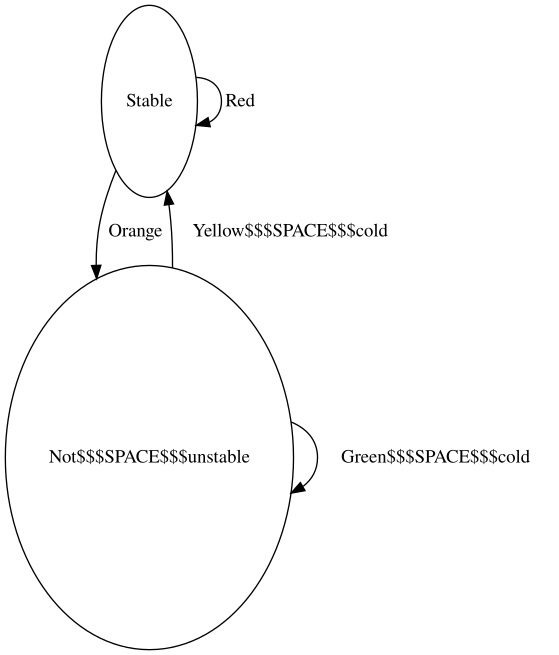
\includegraphics[]{create_bundled_edges_and_vertices_markov_chain.png}
  \caption{
    .svg file created from the create\_bundled\_edges\_and\_vertices\_markov\_chain function 
    (algorithm  \ref{lst:create_custom_vertices_markov_chain}) 
    its .dot file converted from .dot file to .svg using algorithm 
    \ref{lst:convert_dot_to_svg}
  }
  \label{fig:create_bundled_edges_and_vertices_markov_chain.svg}
\end{figure}

%%%%%%%%%%%%%%%%%%%%%%%%%%%%%%%%%%%%%%%%%%%%%%%%%%%%%%%%%%%%%%%%%%%%%%%%%%%%%%%%
\section{Creating $K_{3}$  with bundled edges and vertices}
\label{subsec:create_bundled_edges_and_vertices_k3}
%%%%%%%%%%%%%%%%%%%%%%%%%%%%%%%%%%%%%%%%%%%%%%%%%%%%%%%%%%%%%%%%%%%%%%%%%%%%%%%%

Instead of using edges with a name, or other properties, here we use a bundled
edge class called \verb;my_bundled_edge;.

\subsection{Graph}

We reproduce the $K_{3}$ with named edges and vertices of chapter 
\ref{subsec:create_named_edges_and_vertices_k3}, 
but with our bundled edges and vertices instead:

\begin{figure}
  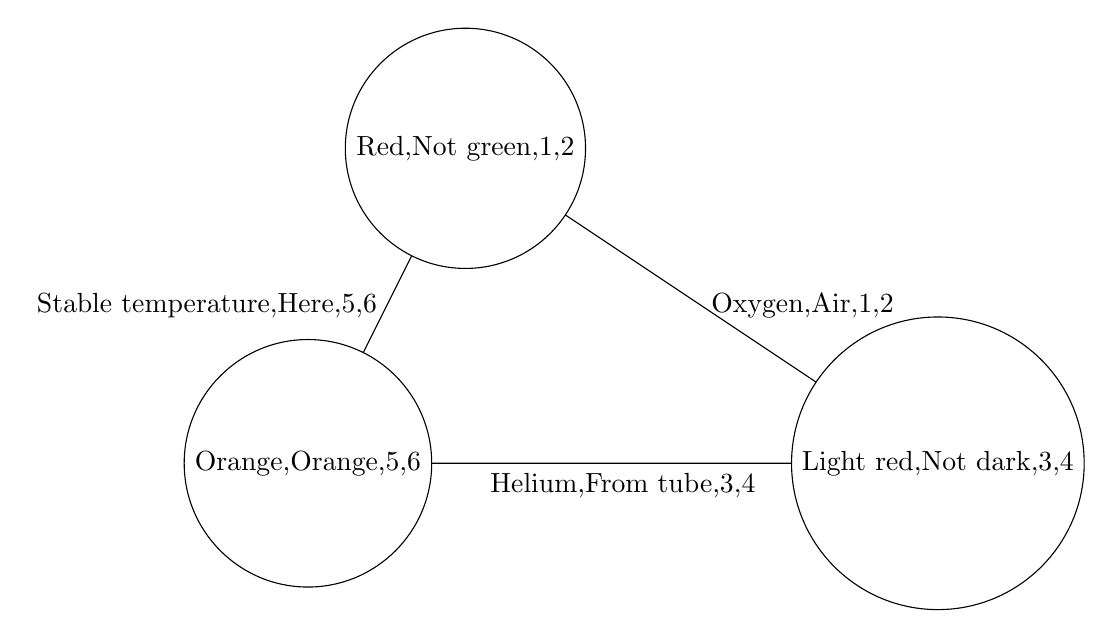
\begin{tikzpicture}
    \draw[] 
      (2,4) node[draw=black,fill=white,shape=circle,text=black] {Red,Not green,1,2}
       -- (5,2) node[anchor=west] {Oxygen,Air,1,2} 
       -- (8,0) node[draw=black,fill=white,shape=circle,text=black] {Light red,Not dark,3,4} 
       -- (4,0) node[anchor=north] {Helium,From tube,3,4} 
       -- (0,0) node[draw=black,fill=white,shape=circle,text=black] {Orange,Orange,5,6} 
       -- (1,2) node[anchor=east] {Stable temperature,Here,5,6} 
       -- (2,4)
    ;
  \end{tikzpicture}
  \caption{$K_{3}$: a fully connected graph with three named edges and vertices }
  \label{fig:create_bundled_edges_and_vertices_k3}
\end{figure}

\subsection{Function to create such a graph}

\lstinputlisting[
  caption = Creating $K_{3}$ as depicted in figure \ref{fig:named_edges_and_vertices_k3},
  label = lst:create_bundled_edges_and_vertices_k3_graph
]{create_bundled_edges_and_vertices_k3_graph.impl}
\index{Create bundled edges and vertices K3 graph}

Most of the code is a slight modification of algorithm 
\ref{lst:create_named_edges_and_vertices_k3_graph}.
In the end, the my\_edges and my\_vertices are obtained as the graph its
property\_map and set with the \verb;my_bundled_edge; 
and \verb;my_bundled_vertex; objects.

\subsection{Creating such a graph

Here is the demo:

\lstinputlisting[
  caption = Demo of the create\_bundled\_edges\_and\_vertices\_k3\_graph function (algorithm \ref{lst:create_bundled_edges_and_vertices_k3_graph}),
  label = lst:create_bundled_edges_and_vertices_k3_graph_demo
]{create_bundled_edges_and_vertices_k3_graph_demo.impl}

\subsection{The .dot file produced}

\lstinputlisting[
  caption = .dot file created from the create\_bundled\_edges\_and\_vertices\_markov\_chain function (algorithm \ref{lst:create_bundled_edges_and_vertices_k3_graph}) converted from graph to .dot file using algorithm \ref{lst:save_graph_to_dot},
  label = lst:create_bundled_edges_and_vertices_k3_graph.dot
]{create_bundled_edges_and_vertices_k3_graph.dot}

\subsection{The .svg file produced}

\begin{figure}[!htbp]
  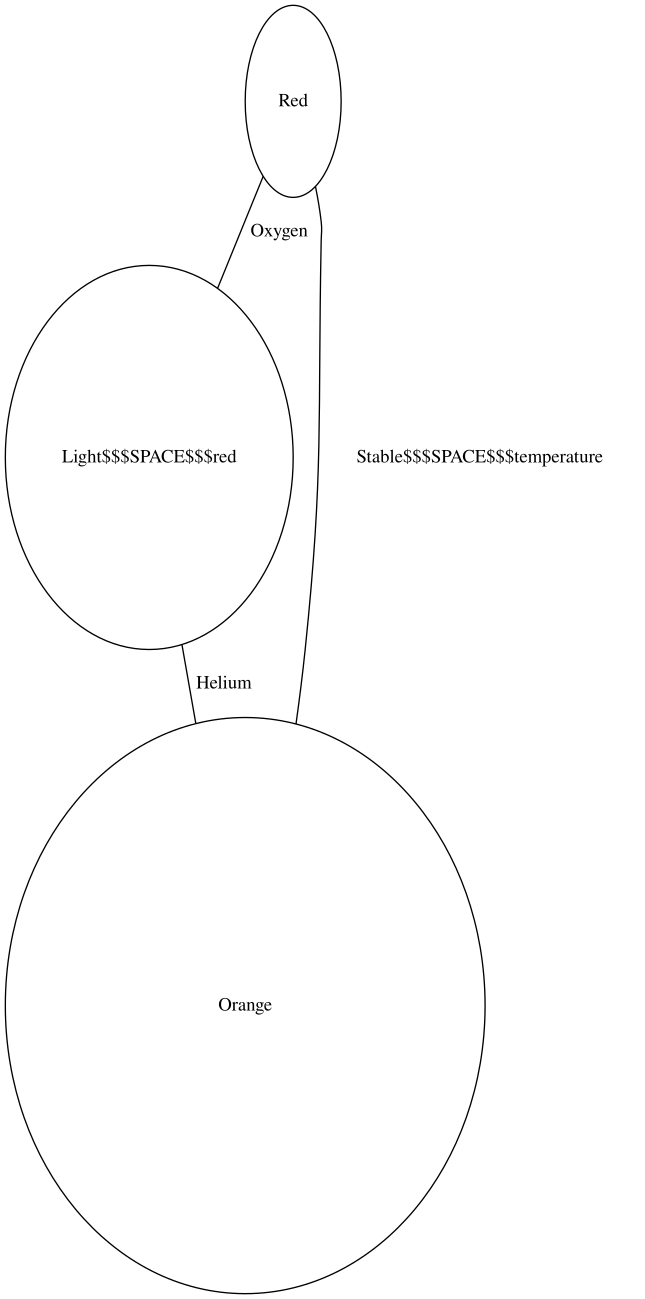
\includegraphics[]{create_bundled_edges_and_vertices_k3_graph.png}
  \caption{
    .svg file created from the create\_bundled\_edges\_and\_vertices\_k3\_graph function
    (algorithm \ref{lst:create_custom_vertices_markov_chain}) 
    its .dot file, converted from .dot file to .svg using algorithm 
    \ref{lst:convert_dot_to_svg}
  }
  \label{fig:create_bundled_edges_and_vertices_k3_graph.svg}
\end{figure}

